%--------------------------------------------------------------------
%
%Mustervorlage fuer eine Aufgabe
%
%--------------------------------------------------------------------
%
%Ueberschreiben der automatisch erzeugten Aufgabennummer
%Die folgende Aufgabennummer ergibt sich aus dem Stand des
%Z�hlers + 1
%\setcounter{chapter}{0}
%
\chapter{Methodology and Implementation}\label{chap:implementation}
%
%
%

As mentioned previously, this project consists of several components that run in unison to each other. Each component can be thought of as a building block to form a wall. To successfully build the wall, each block must be carefully placed so that it effectively supports the next. These components are ROS, Lego Boost robot, Localization algorithms, and motion control algorithm.\\
In this chapter, the implementation and methodology of each component will be explained. 

\section{ROS Software Architecture}
For a better understanding of the developed ROS software, it is important to describe its architectural design and explain the connection between its different components. This section describes the overall ROS software architecture, as mentioned in \cite{joseph_learning_2018} and also the architecture of the implemented software.
 
In general, the architecture of any software which is based on ROS can be divided into two main layers. The first layer is the ROS computation graph. This computation graph contains nodes, topics, messages, and other components. The second layer is the ROS filesystem, which contains all files and packages of the software. A general example of the architecture design of a  software-based on ROS is shown in \ref{fig1}.  The components of each layer of the software are described and discussed in detail in the following subsections. 

\begin{figure}[ht]
	\centering
	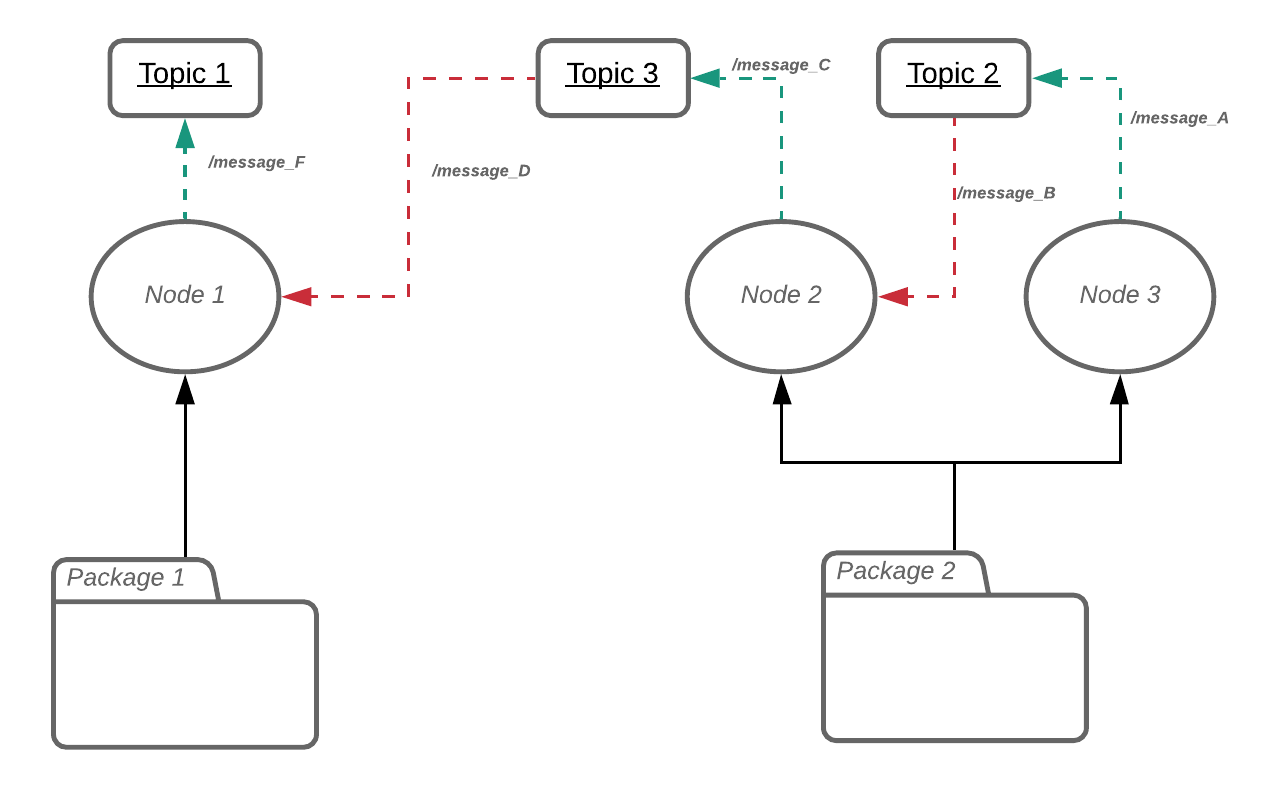
\includegraphics[width = 0.8\textwidth, frame]{./Bilder/UML_Architecture.png}			\caption{ROS architecture design}
	\label{fig1}
\end{figure}


\subsection{ROS Filesystem}


The top component of the filesystem is the catkin workspace, which contains all used ROS packages. Beneath the catkin workspace come the packages. The packages provide different tools and libraries, which could be used and configured to accomplish the desired functionalities. Each package contains messages, data types, services, and most importantly, executable files and launch files \cite{joseph_learning_2018}. The executable files written either in C++ or in Python, are used to initialize ROS nodes. The launch files are used to configure and launch specific nodes. Since ROS is an open-source tool, all its packages can be found through the ROS Software Browser. During installation, there are some default packages that are recommended while downloading ROS. Other than this, all remaining packages must be downloaded or cloned individually from the Software Browser or alternatively be made from scratch. The following figure \ref{fig2} clearly demonstrates all the packages used in this project and the nodes that they include. The directory structure of the whole system is displayed in appendix \ref{chap:app2}


\begin{figure}[ht]
	\centering
	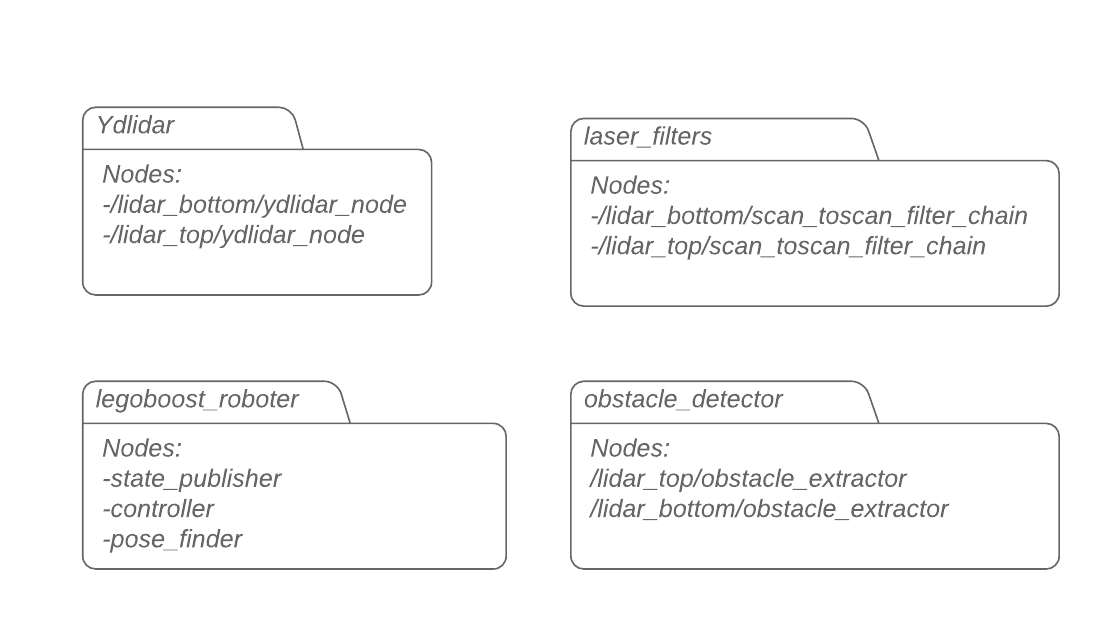
\includegraphics[width = 0.8\textwidth, frame]{./Bilder/UML_Packages.png}			\caption{ROS packages of the project}
	\label{fig2}
\end{figure}






Packages needed to be installed to support the default ROS packages are: 
\begin{enumerate}
\item \textbf{Ydlidar Package:} This package should be installed first. It supports the YdlidarX2  triangulation laser scanner, which is developed by Shenzhen EAI Technology Co. It contains all the executable files that process the laser scanner data and publishes it as a LaserScan message to a topic. The nodes created in these packages are the /lidar-bottom/ydlidar-node and the /lidar-top/ydlidar-node, which contain information about the bottom and top laser scanners, respectively. Further information about the nodes is discussed in the computation graph section \ref{subsec:computationGraph}.
\item  \textbf{The Laser-Filters Package:} As mentioned in \cite{noauthor_laser_nodate}, this package is responsible for adjusting messages of type LaserScan obtained from the triangulation laser scanner by using predefined filters so that it is suitable for later processing. 
 Another option is to use pointCloud messages, but this option is not required as the laser scanner publishes messages of type laserscan and not point-cloud. This package includes a node called scan-toscan-filter-chain, which is a pipeline of filters defined by the user. It is useful for instances such as removing laser scan points of the wall to concentrate only on the robot laser scan data.
\item  \textbf{The Obstacle Detector Package:} As seen in \cite{przybyla_obstacle_detector_2020}, this package is initially used for obstacle detection and tracking by using laser scan data from laser scanners. However, in our case, this package is used to detect the robot. The node used in this package is called the obstacle-extractor node. This package also has a user-defined message type called "Obstacle" which includes the position of the obstacle in the XYZ plane. It also has nodes to visualize the obstacles in rviz. 
\item  \textbf{The Legoboost-Roboter Package:} Unlike the other packages, this one is made from scratch and contains all the information about the robot. This package consists of three main components; the controller, pose detector, and state publisher, each of which has a specific function. The state publisher consists of a node responsible for publishing the robots' frames and contains its URDF file. The pose detector is essentially a node that calculates the position and orientation of the robot using data collected from the obstacle collector. And lastly, the controller, which has a node that is responsible for the motion control of the robot.
\end{enumerate}





\subsection{ROS Computation Graph}\label{subsec:computationGraph}



This section will go more in-depth on the computation graph layer for a better understanding of the software architecture as described in \cite{joseph_learning_2018}. The computation graph is responsible for the connection between these components and the way the information is exchanged between these components. ROS node is one of the main components of the computation graph. It is responsible for computing a specific functionality or task.  ROS Nodes are connected together through topics or services. They could subscribe to topics to get the information from these topics and use this information to perform a specific task. They can also publish information to topics to post-process this information. Information that is exchanged between topics is called a message. Messages types can be either built-in, for example String or Bool, or can be defined by the user. Figure \ref{fig3} shows the nodes used in this software and how they are interconnected. Any item within a square notion that this item is a topic, however, an item within a circle relates to a node. This figure is generated by the rqt tool from ROS. This is a framework that is used for GUI purposes. 



\begin{figure}[ht]
	\centering
	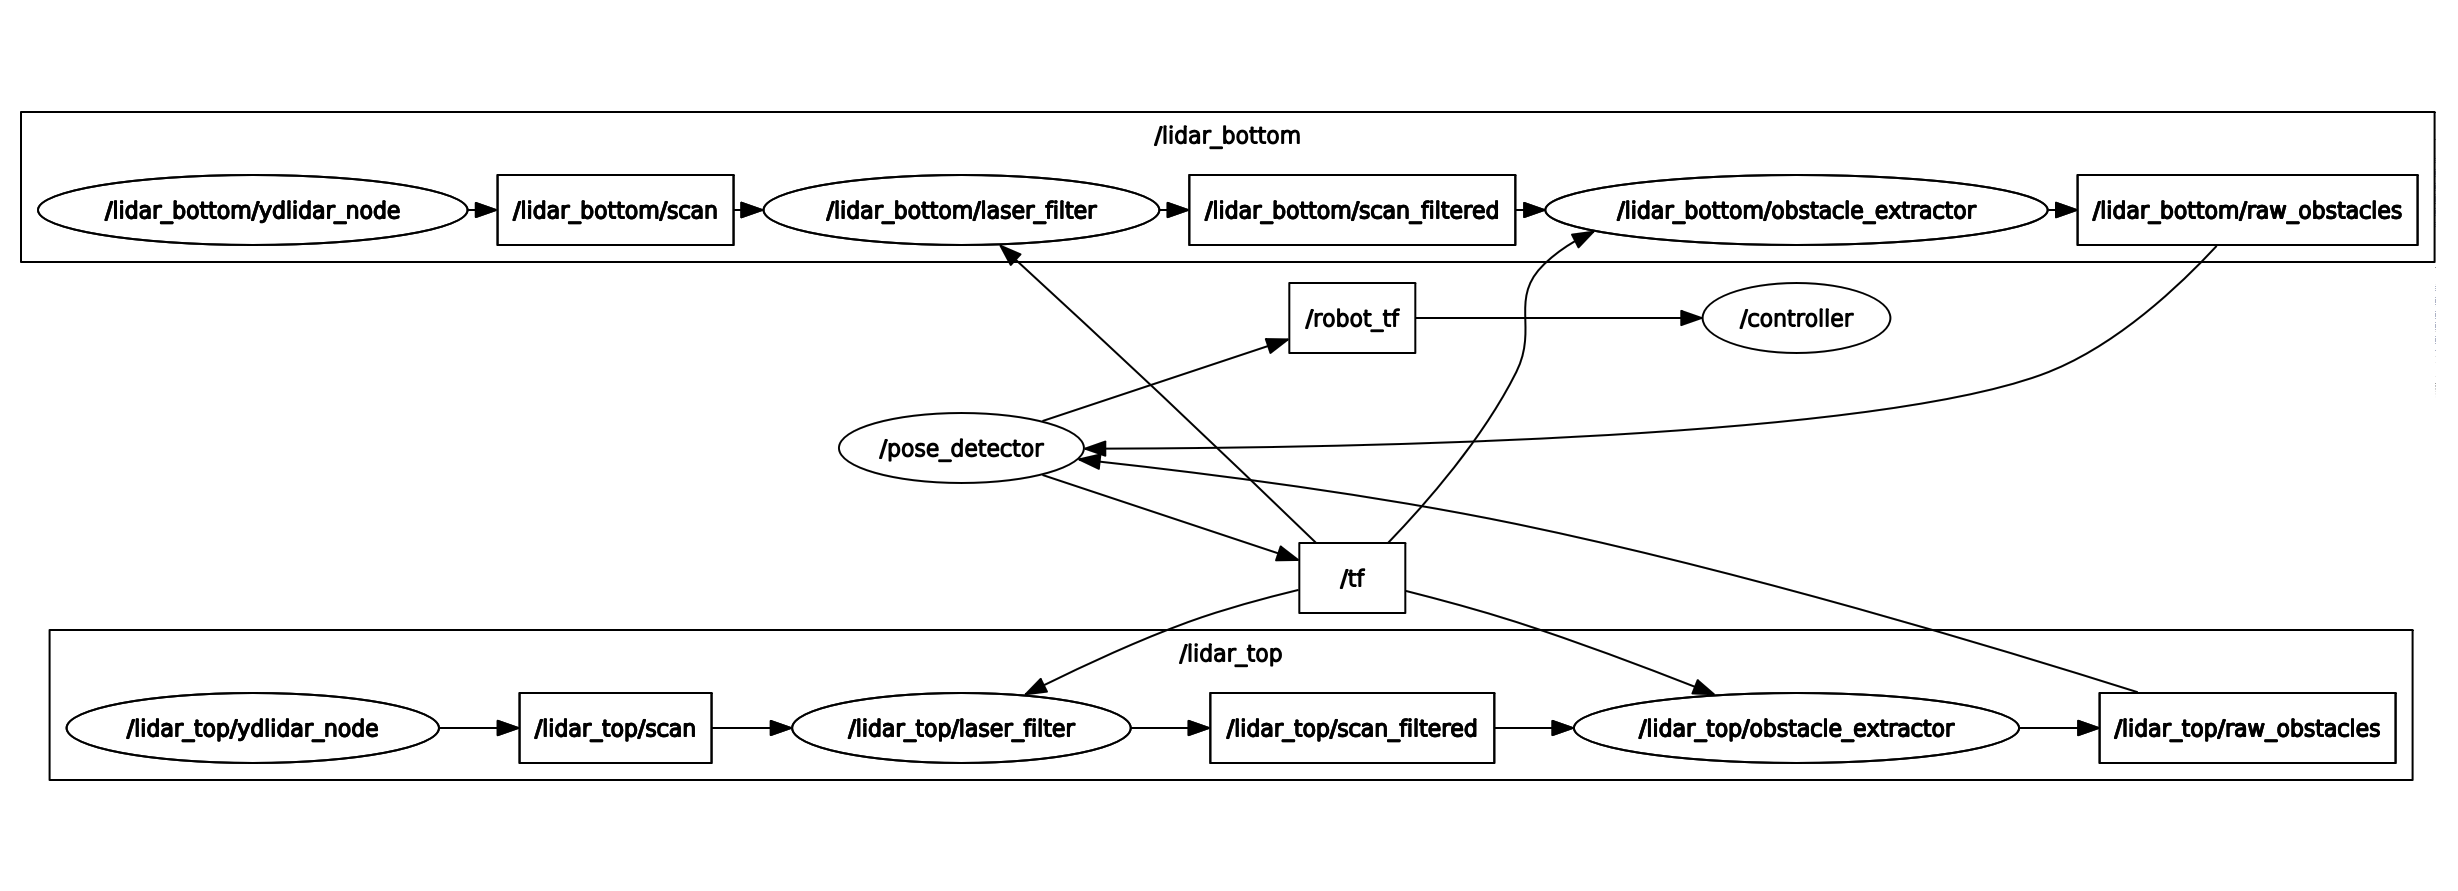
\includegraphics[width = 1.0\textwidth, frame]{./Bilder/rosgraph_nodes.png}			\caption{Relation between the nodes used in the project}
	\label{fig3}
\end{figure}


Since there are two laser scanners and the data of each laser scanner must be processed individually, it is essential to launch separate nodes for each one. This can be done by using the attribute "ns" in the launch file. By using this attribute, an instance of the node can be created in a user-defined namespace so that separate nodes are initiated. Figure \ref{fig3} shows these two namespaces, which are named "lidar\_bottom" and "lidar\_top".



As described in the previous figure, the nodes are:
\begin{enumerate}
\item \textbf{State-Publisher:} This node is responsible for publishing the joint states and transformers of the robot.

\item \textbf{lidar\_bottom/ydlidar\_node and lidar\_top/ydlidar\_node:} These nodes publish messages of type LaserScan to the topics "lidar\_bottom/scan" and "lidar\_top/scan" respectively. As defined in \cite{noauthor_sensor_msgs_nodate}, a LaserScan message in ROS is defined in sensor\_msgs package and it contains information about laser scanner scans such as the ranges of each angle as well as the scan time and maximum and minimum range. 

\item \textbf{lidar\_bottom/scan\_filter and lidar\_top/scan\_filter}: These nodes subscribe to the scan topics which are published from the ydlidar\_node and publish a filtered LaserScan message to the topics "lidar\_bottom/filtered\_scan" and "lidar\_top/filtered\_scan". The scan\_filter nodes in each laser scanner use LaserScanBoxFilter, which exclude scan points that are outside a defined room\citep{noauthor_laser_nodate}. The room is defined by two points in an XYZ-space. This is important to exclude the scan points of the room's walls. By doing this, only the scan points of the robot are going to be considered. Figure \ref{fig4} shows the plan view of the room, and the position of the laser scanners as well as the coordinates of the room. The XY coordinate of the laser scanners is (0,0), and the room's length as well as the room's width, is 1.6 meters. The laser scanner is placed 15 cm apart from the wall in both x and y directions. It's therefore concluded that  $P_{min}$ = (0.15,-0.15) and $P_{max}$ = (-1.45,1.45). 
\begin{figure}[ht]
	\centering
	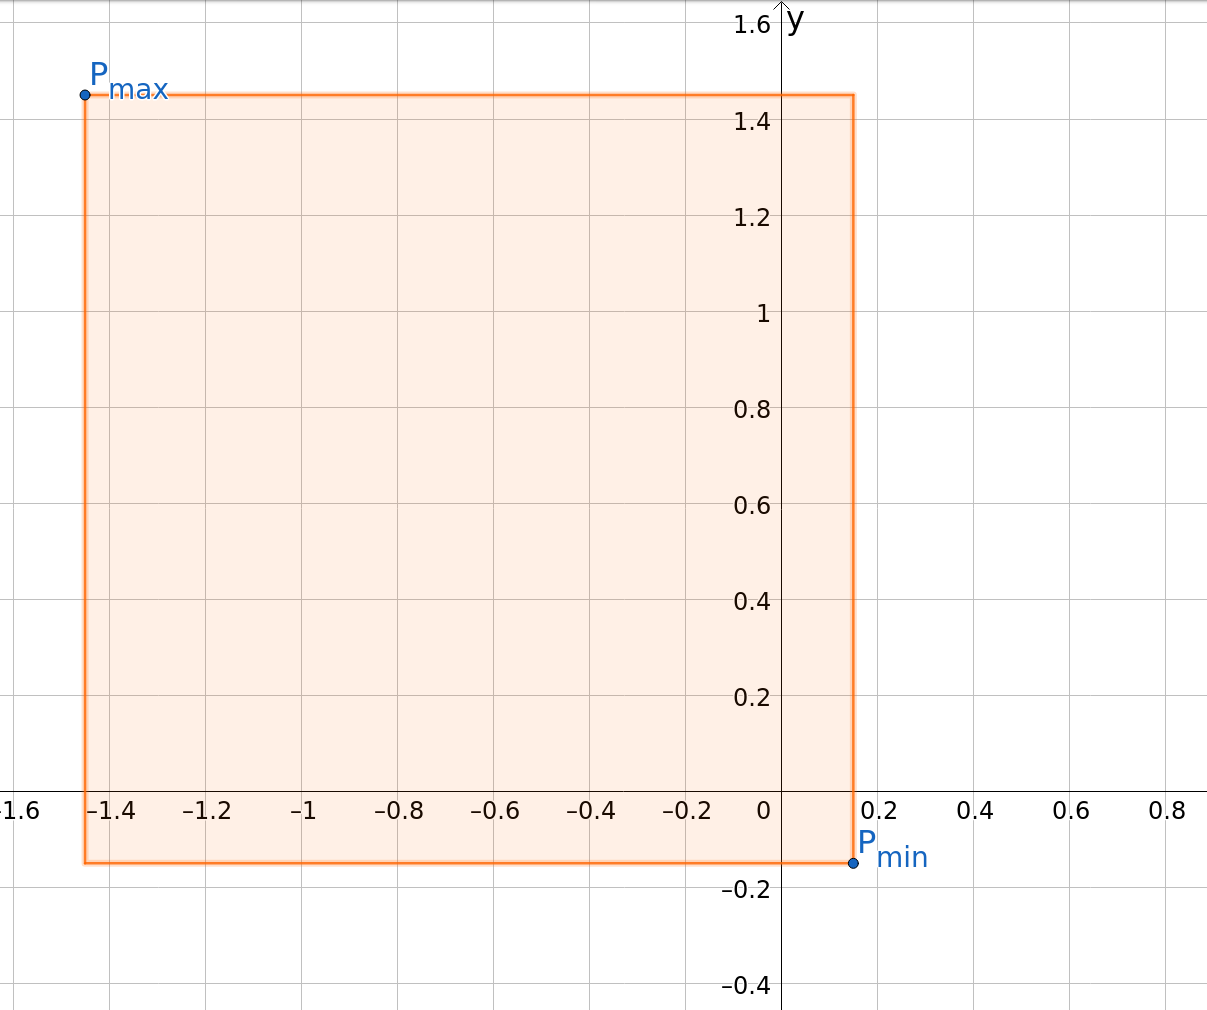
\includegraphics[width = 0.8\textwidth, frame]{./Bilder/room1.png}			\caption{Plan view of the room}
	\label{fig4}
\end{figure}

\item \textbf{lidar\_top/obstacle\_extractor and lidar\_bottom/obstacle\_extractor:} subscribe to the scan\_filter topic of each laser scanner and  publish messages of type Obstacles to the topics "/lidar\_top/raw\_obstacles" and "/lidar\_bottom/raw\_obstacles."

\item \textbf{Pose\_Detector:} This node subscribes to the raw\_obstacle topic of each laser scanner and publishes the pose of the robot as a transformer message to the topic "robot\_tf". 

\item \textbf{Controller:} This node subscribes to the robot pose and calculates the velocities of the left and right wheels. Then it sends velocity commands to the control unit.\\
The implementation of obstacle extractor nodes, as well as the pose\_detector node and controller node is discussed in further sections.
\end{enumerate}

\section{Model Architecture and Visualization}

The design and visualization of the required model are two other building blocks that are essential for the successful completion of the project. Visualizing the components of the model using visualization tools that are provided by the ROS is important for tracking results and debugging the robot's motion. The designed model consists of three main components, namely the robot, the laser scanners, and the room. In the first subsection, the specifications and requirements of each component are explained in detail. Based on these requirements and specifications, the design of each component is going to be explained. In the second subsection, the visualization of the model in rviz is explained as well as the implementation of the robot's URDF.  

\subsection{Model Design}\label{subsec:ModelDesign}

\textbf{System Requirements:\\}
The first requirement of the system concerns the robot and laser scanner design. These two components must have a design that facilitates the localization process of the robot for the triangulation laser scanners to detect the position as well as the orientation of the robot. \\
The second requirement is that the room design must be rectangular or square-shaped. Besides, the floor of the room must be a whiteboard, and the laser scanners must be placed at a corner of the room. Lastly, the area of the room must be large enough for the robot to navigate within, yet not too large to ensure precise detection of the robot pose.

\textbf{System Specifications:\\}
Some of the robot specifications are already known since they are closely tied to the Lego Move Hub specifications because it is the central control unit of the robot. However, other specifications must be included that are based on the requirements discussed above. These are listed below.
\begin{enumerate}
\item Communication Protocol:
Move Hub uses a Bluetooth Low Energy (BLE) processor for the communication between the control unit and the PC. The Bluetooth communication is based on GATT protocol.
\item Steering system:
Since Move Hub has two separated motors, each controlled individually, then the steering system of the robot is differentially steered. This steering system is nonholonomic.
\item Robot design:
The design of the robot is related to the first requirement mentioned previously. After several trials with different designs, a specific design was achieved as follows:
\begin{itemize}
\item The robot has two cylinders with the same radius. One of these cylinders is placed at the front and the other at the back of the robot.
\item The cylinders are placed in different YZ planes. 
\item  The cylinders are wrapped with papers in order to decrease data loss. This papers are diffusely reflective. 
\end{itemize}
The following figure \ref{fig:fig5} shows the design of the robot. The design is made by Mecabricks.com, which is a web service to design models using Lego bricks. 
\begin{figure}[ht]
\begin{subfigure}[c]{0.5\textwidth}
  \centering
  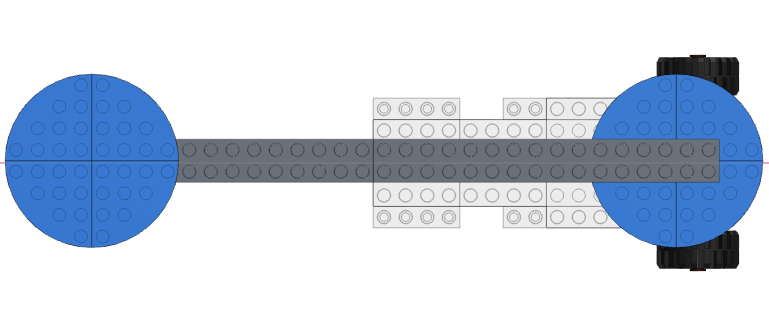
\includegraphics[width=1\linewidth]{./Bilder/Robot_Top.png}
  \caption{Plan view}
  \label{fig5:sfig1}
\end{subfigure}%
\begin{subfigure}[c]{0.5\textwidth}
  \centering
  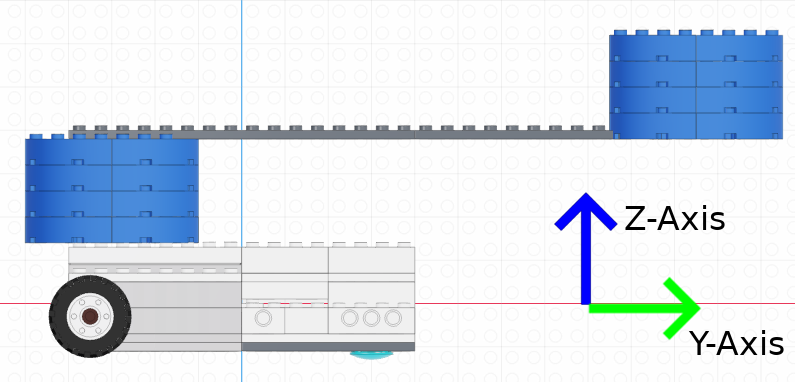
\includegraphics[width=0.8\linewidth]{./Bilder/Robot_Side1.png}
  \caption{Side view}
  \label{fig5:sfig2}
\end{subfigure}
\caption{Plan and side view of the robot.}
\label{fig:fig5}
\end{figure}
\item Laser scanners design:
The system has two laser scanners each determine a different cylinder. The laser scanners are placed on each other with the same orientation so that the x and y-axis of both laser scanners are identical. The laser scanner which is placed on top is on the same scanning plane as the cylinder which is placed on top. The same applies to the other laser scanner. 
\item Room design:
The fifth specification is the design of the room and is related to the second requirement mentioned in the requirements above. To design the room, it's important to consider two aspects. The first one is  the laser scanner's specifications, which are discussed in section \ref{sec:lidar}. The second aspect is the ability of the obstacle detector algorithm, which is used to detect the cylinders. By considering these aspects, the maximum area of the room can be determined as follows.\\
The angle increment of the laser scanner is 0.72 $\frac{degrees}{step}$. To detect the circular obstacles  an algorithm called "Obstacle Detector" is used. The implementation of this algorithm will be discussed in \ref{circDet}. However, for using the obstacle detector algorithm at least five laser beams of the object must be valid. The first and the last beam values are the tangents of the cylinder. The minimum valid angle between those tangents indicates the maximum range between the laser scanner and the obstacle. This angle is calculated using equation \ref{eq0}

\begin{equation}\label{eq0}
\theta_{min} = i \cdot (R_{min}-1)
\end{equation}
where \hspace{15mm} $i$  =  angle increment\\ 
	  \hspace*{25mm} $R_{min}$  =  minimum number of ranges

The challenge is to find this maximum length using this angle. This can be done by utilizing basic geometry rules using the angle found. The following figure \ref{fig6} shows circle B, which has a radius $r$. The tangents of the circle are connected to the same point $A$. Theta is the angle between the tangents. 

\begin{figure}[ht]
	\centering
	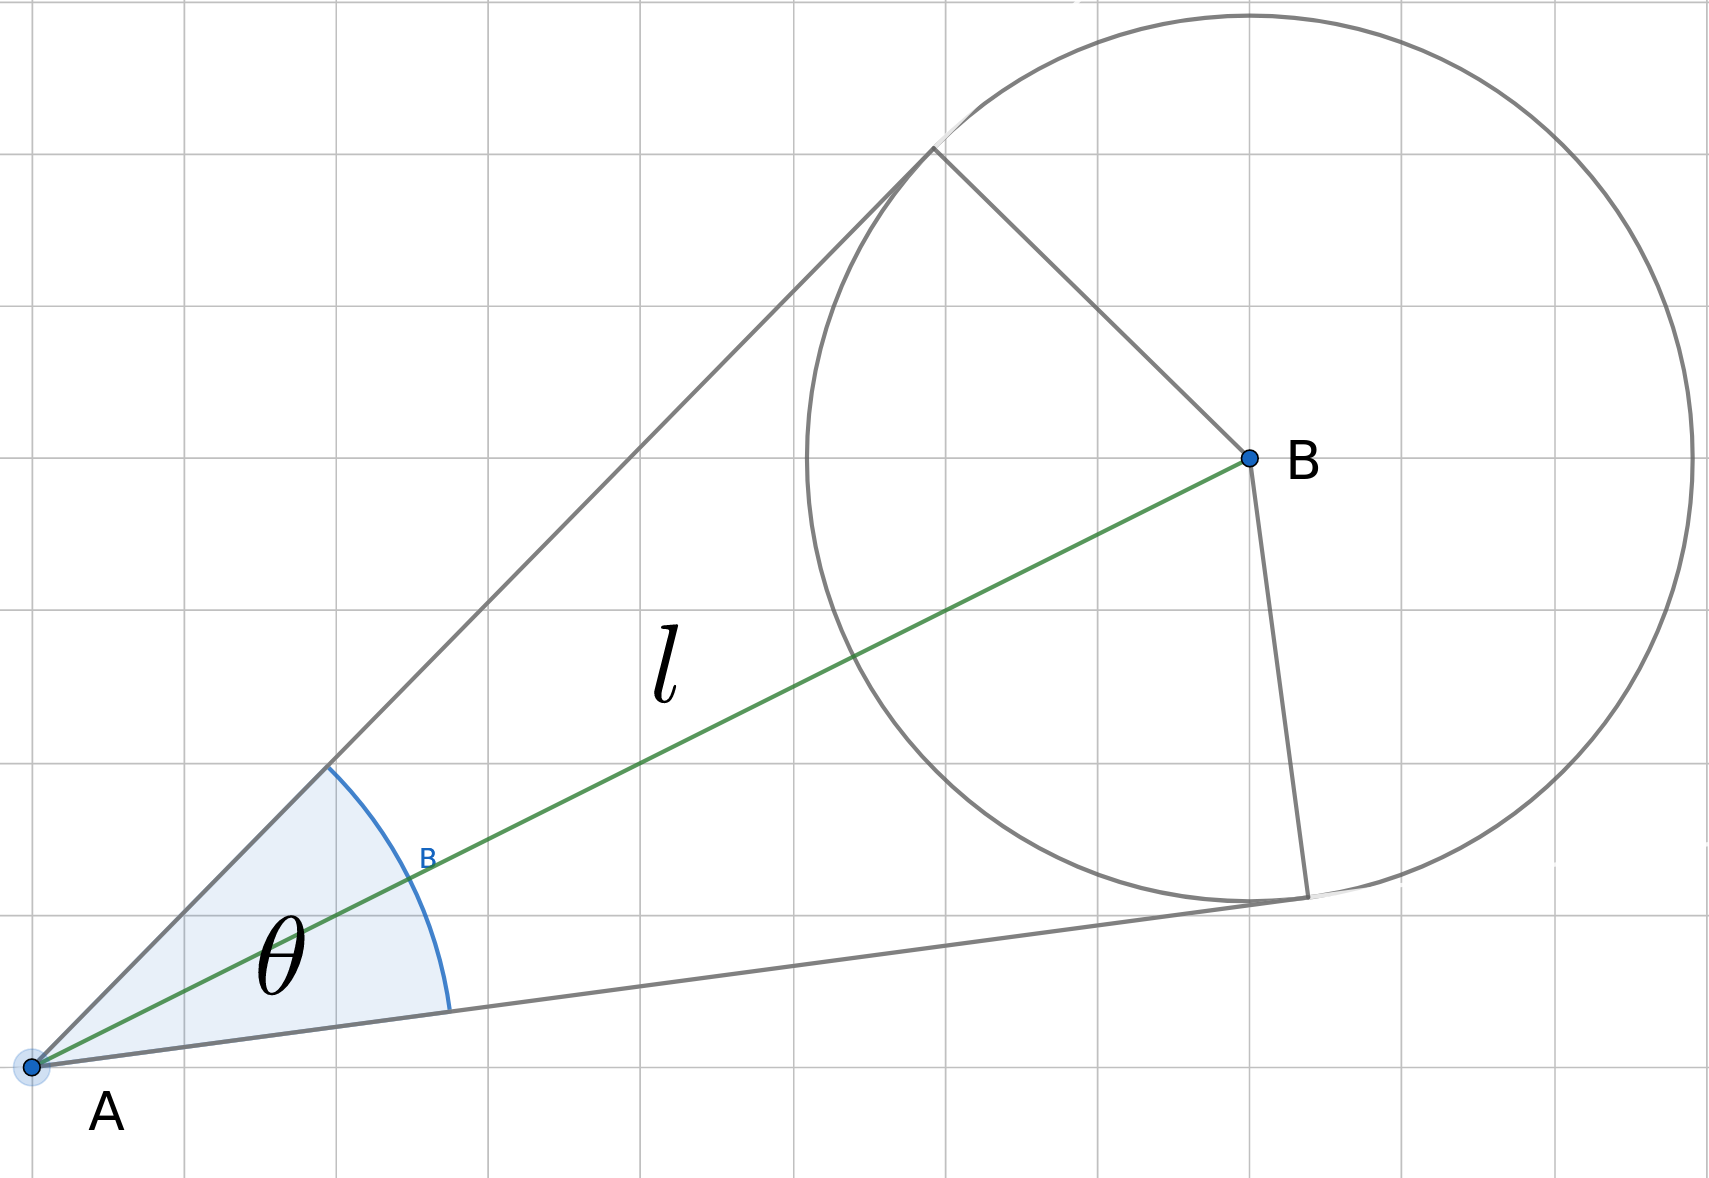
\includegraphics[width = 0.6\textwidth, frame]{./Bilder/geogebra.png}			\caption{The Relation of the length between external point and center of a circle and the angle between circle tangents to this point}
	\label{fig6}
\end{figure}


The length $l$ can be calculated as follows:
\begin{equation} \label{eq1}
l= \frac{r}{sin(\frac{\theta}{2})}
\end{equation}

by substituting theta from equation \ref{eq0} in equation \ref{eq1}
\begin{equation} \label{eq2}
l_{max} = \frac{r}{sin(\frac{i \cdot (R_{min}-1)}{2})}
\end{equation}
where \hspace{15mm} $i = 0.72 \hspace{1mm}\frac{degree}{step}$\\ 
	  \hspace*{25mm} $R_{min} = 5$ steps
	  
From this equation the room dimensions can be specified. By using cylinders with radius $r$ = 62 mm. Then $l_{max}$ = 2.5 m. The maximum distance in the room is the diagonal. The length of each side of the room could be calculated by using the following equation:
\begin{equation} \label{eq3}
a = \frac{l_{max}}{\sqrt{2}} = 1.768 m
\end{equation}
Nevertheless, the range of error must be calculated for the previous analysis. Since the used triangulation laser scanner has a relative error of 1.5\% for any distance between 0.5 m and 6m, and since there are 2 different laser scanners, then FRAGE(Error calculation)
\end{enumerate}

\subsection{Model Visualization}
Visualizing the robot and the other components of the system using visualization tools that are provided by ROS is important for watching the results and monitoring the robot motion. The visualization tool used in ROS applications is called RViz, which is a GUI used to subscribe to topics and visualize the data in these topics. RViz contains specific display types for specific message types. For example, LaserScan display type displays the data from a sensor\_msg::LaserScan message. However new display types could be added by using user-defined plugins. For example an obstacle display type is added to Rviz using a user-defined plugin. Another display type is the Robot Model, which represents the robot pose depending on its URDF. The URDF is an XML file which describes the joints and the links of the robot and the relation between them \cite{noauthor_urdf_nodate}.




The next step is to write the URDF file of the LegoBoost robot. It simply consists of 4 links and 3 joints. The first joint is the base joint, which connects between two links, namely the base footprint which is the parent link, and the base link which is the child link. As defined in \cite{noauthor_coordinate_nodate}, the base footprint demonstrates the position of the robot at the ground level, while The base link is the position of the center of mass of the robot which is placed above the base footprint. These two links are connected through a fixed joint named base joint. The base joint is fixed since it doesn't have any degree of freedom. The second joint is the right wheel joint, which connects the base link to the right wheel link. The last joint is the left wheel joint, which connects between the base link and the left wheel link. The hierarchy of the URDF  and the connection between the different links and joints is shown in figure \ref{fig7}. This figure is generated by urdf\_to\_graphviz tool.

\begin{figure}[ht]
	\centering
	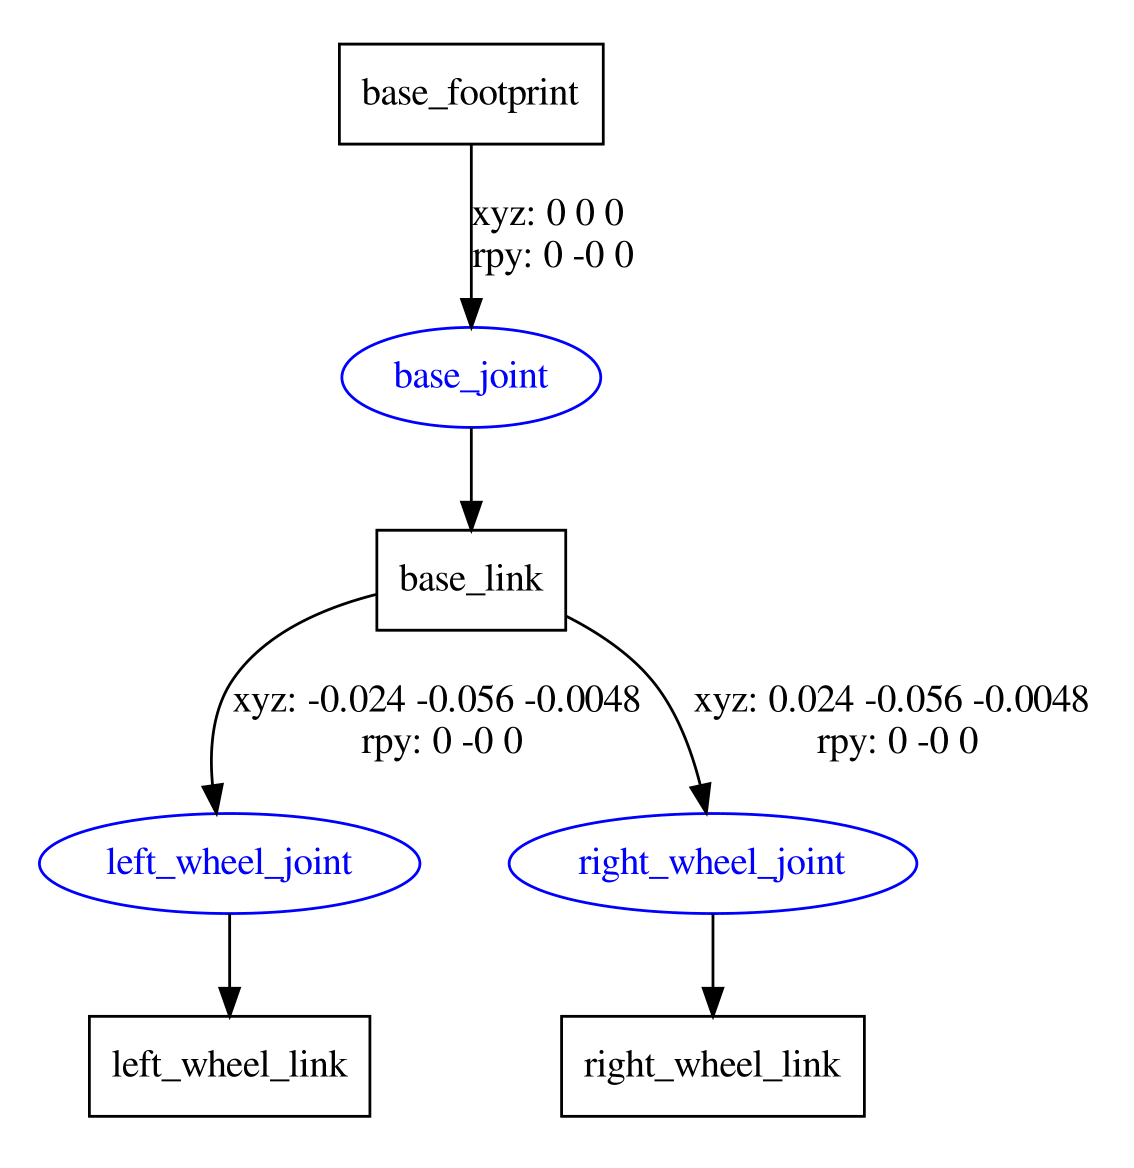
\includegraphics[width = 0.6\textwidth, frame]{./Bilder/legoboost_robot.png}			\caption{Graphical demonstration of LegoBoost URDF}
	\label{fig7}
\end{figure}


Each link in the URDF file can contain visual properties. The visual properties could be used for a better visualization of the robot. The geometry of both right and left wheel links are implemented in the URDF as cylinders with the same radius of the robot's wheels. The base link geometry is implemented as a box with the same dimensions of the robot.\\
After implementing the URDF file, the next step is to set up the Rviz tool and add all the required display types, which are:

\begin{itemize}
\item Robot model: This displays the URDF of the robot.
\item LaserScan: This displays the scan data of the laser scanners. A LaserScan display type is added for each laser scanner.
\item Obstacles: This displays the cylinders on the robot. An obstacle is added to each cylinder. Each cylinder is colored differently, namely red for the top cylinder and blue for the bottom cylinder. 
\item TF: This displays the TF transform hierarchy of the model. 
\end{itemize} 
The final visualization of the whole model in RViz is shown in figure \ref{fig8}. The frames of the laser scanners as well as the robot are demonstrated. The red and white points demonstrate the laser scans of the laser scanners and the red-green cylinder shows the back cylinder of the robot. Lastly, the grey-blue cylinder demonstrates the front cylinder of the robot. 

\begin{figure}[ht]
	\centering
	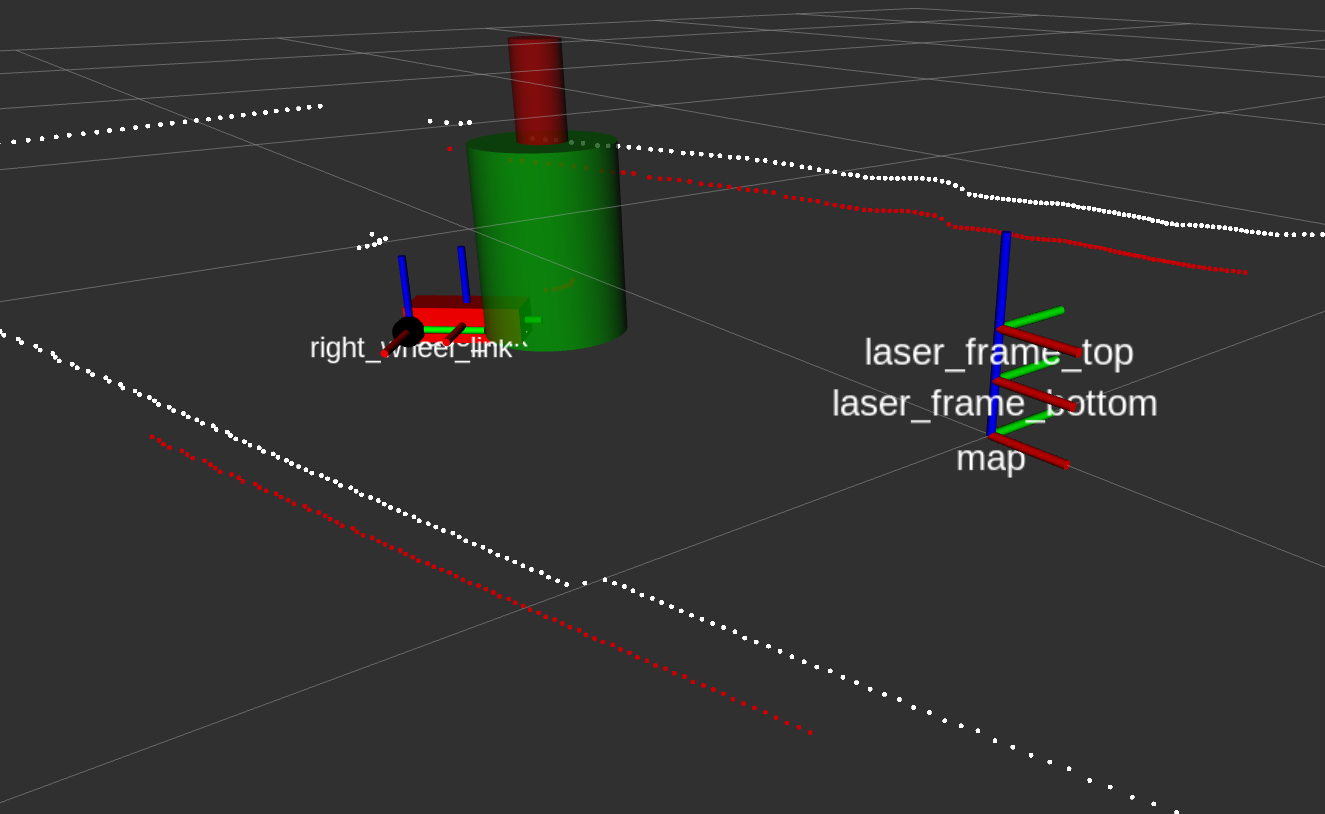
\includegraphics[width = 0.9\textwidth, frame]{./Bilder/rviz_screenshot.png}
	\caption{The model visualization in RViz}
	\label{fig8}
\end{figure}

\section{Robot Localization}
Robot localization is another essential building block in the project and the core of the thesis. Under robot localization, two things must be considered. First, is localizing the position of the robot, and second, localizing the orientation of the robot. Both the orientation and the position represent the pose of the robot. Localization in mobile robots context is usually performed by using SLAM algorithms, where a LIDAR or a camera is integrated into the robot to scan the surrounding environment, and the SLAM algorithms are used to build a map of this environment and localize the pose of the robot depending on this map and other inputs like the odometry of the robot \cite{yoonseok_ros_2017}.\\
In contrast to the SLAM algorithms, the method used in this thesis is  different since the laser scanner are not integrated into the robot but fixed in a specific place in the room. From the perspective of the laser scanner, the surrounding environment is still, and only the robot is moving. Using a fixed sensor in the room has an advantage, namely the cost efficiency of the solution by saving the battery of the robot and also by saving the costs of other robot components such as odometry sensors or IMU sensors. In this section, the used methods, which have been used for robot localization, are going to be discussed. 
First, localization using the obstacle detector approach is discussed, then using image processing is discussed, and last using the laser scan matcher approach.

\subsection{Circular Object Detection} \label{circDet}  %8 pages
%1)introduction and explain how the algorithm work   1page
%2)how did I implement the approach to detect the robot pose 6pages
%	2.1 Idea explanation (Geometry)
%	2.2 Code explanation
%3)how accurate is the detection 1 page
%4) conclusion 1 page


Obstacles detection algorithms are essential in robot navigation. Such algorithms are used,e.g., during navigation to avoid obstacles. The obstacle detection algorithm developed in \cite{przybyla_detection_2017} is used for detecting circle-shaped obstacles by using circles geometric properties and the polynomial regression of laser scan data. The main reason for choosing this algorithm is its fascinating efficiency and speed. According to the applied tests mentioned in \cite{przybyla_detection_2017}, the accuracy rate of the circles' detection is 92.53\%, and the average executing time is 16 ms per frame, which is around 50 \si{\hertz}. This is more than twice the publishing rate of the X2 laser scanner, which is 20 \si{\hertz}. This is the advantage of ROS, where a node could be reused and adjusted depending on the requirements or the problem. The main idea of using this algorithm is to detect the cylinders that are placed on the robot. The pose of the robot can be calculated by detecting the exact position of these cylinders in cartesian coordinates form. The implementation of this approach is divided into three main steps. The first step is to find a geometrical solution to the problem. The second step is tuning the obstacle extractor node parameters to fit with the specifications of the robot. The last step is to implement this geometrical solution in an executable file, i.e., C++ or Python.\\
The geometrical problem can be divided into two main problems. The first problem is finding the position of the robot. The position here means the middle point between the front and back cylinders in the XY plane. The second problem is finding the orientation of the robot. In other words, the main question is how to transform the coordinates of the laser scanner to the coordinates of the robot. Figure \ref{fig9} shows an example of the robot coordinates $P_{Robot}$ relative to the laser scanner $P_{Sensor}$. The points $C_{f}$ and $C_{b}$ represent the center of the front and the center of the back cylinders, respectively. The dotted coordinates indicate the laser scanner coordinates after transforming them into the robot's coordinates. 

\begin{figure}[ht]
	\centering
	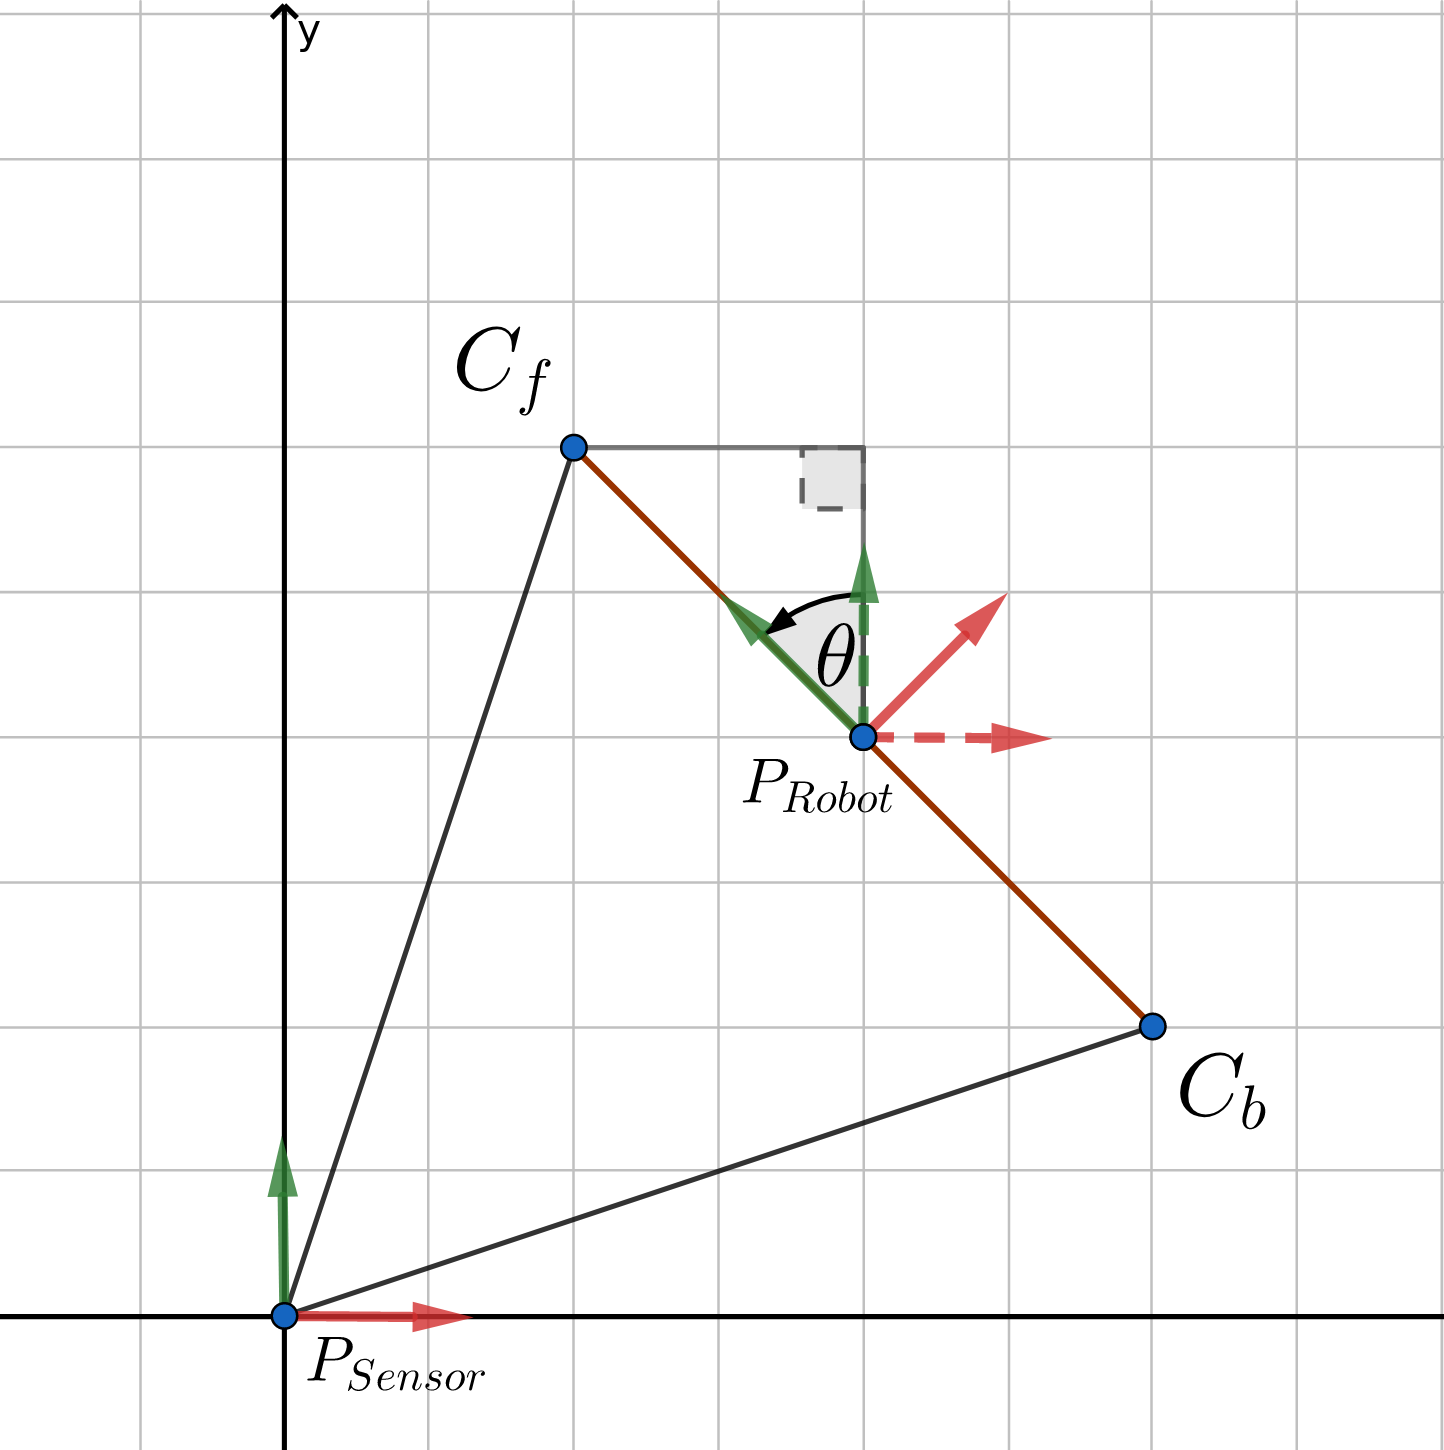
\includegraphics[width = 0.7\textwidth, frame]{./Bilder/geogebra_transform.png}
	\caption{Robot and Sensor coordinates in the room}
	\label{fig9}
\end{figure}

The position of the robot can be obtained by applying the midpoint formula as follows: 
\begin{equation}\label{eq4}
P_{Robot,y} = \frac{C_{f,y}+C_{b,y}}{2}, \hspace{3mm}P_{Robot,x} = \frac{C_{f,x}+C_{b,x}}{2}
\end{equation}


To find the orientation of the robot, the angle $\theta$ must be calculated. By using the trigonometric function:

\begin{equation*}
tan(\theta)= \frac{opposite}{adjacent}
\end{equation*}
then,	  
\begin{equation}\label{eq5}
\theta= arctan(\frac{C_{f,y} - P_{Robot,y}}{C_{f,x}-P_{Robot,x}})
\end{equation}  

After determining the geometrical solution of the problem and deriving the required equations to find the pose of the robot, the next step is to implement this solution in a ROS node. The first thing to be considered in the implementation is setting the obstacle extractor node parameters. This node is responsible for extracting the cylinders' position and publish them for further processing. The definition of each parameter is extracted from  \cite{przybyla_obstacle_detector_2020} and listed below:

\begin{table}[h]
\centering
\begin{tabular}{|| c | l | c ||} 
 \hline
 Parameter & Definition & Value \\ [0.5ex] 
 \hline\hline
 active & Active/Sleep mode & true \\ 
 \hline
 use\_scan & Use laser scan messages & true \\
 \hline
 min\_group\_points & \makecell[l]{Minimum number of points comprising a group to \\ be further processed} & 5 \\
 \hline
 max\_group\_distance & \makecell[l]{If the distance between two points is greater than \\ this value, start a new group} & 0.06 \\
 \hline
 max\_merge\_separation & \makecell[l]{If the distance between obstacles is smaller than \\ this value, consider merging them} & 0.3 \\
 \hline
 radius\_enlargement & Artificially enlarge the circles' radius by this value & 0  \\ [1ex] 
 \hline
\end{tabular}
\caption{The definition of obstacle\_extractor node parameters}
\label{table:1}
\end{table}

By considering the requirements discussed in \ref{subsec:ModelDesign}, the minimum\_group\_points parameter is set to 5. To find a proper value of the parameter maximum\_group\_distance, the maximum length of the room calculated in section \ref{subsec:ModelDesign} must be considered. At this distance, the triangulation laser scanner detects only five points of the cylinder. The distance between any two points, in this case, can be calculated using the formula of a circle's cord as follows:

\begin{equation*}\label{eq6}
c = r \cdot crd(\alpha)
\end{equation*}  

\begin{equation}\label{eq7}
c= 2r \cdot sin(\frac{\alpha}{2})
\end{equation}  

where \hspace{15mm} $\alpha$ is the angle between two points from circle center perspective. \\ 
	  \hspace*{27mm} $c$ is the distance between these two points.
	  
By using equation \ref{eq0}, the angle $\alpha$ can be calculated as follows:

\begin{equation}\label{eq8}
\alpha = \frac{180-(R_{min}-1)\cdot i}{R_{min}-1}
\end{equation}  

By substituting \ref{eq8} in \ref{eq7}, then

\begin{equation*}\label{eq9}
c = 2r \cdot sin(\frac{1}{2} \cdot \frac{180-(R_{min}-1)\cdot i}{R_{min}-1})
\end{equation*}  
This can be simplified into

\begin{equation}\label{eq10}
c = 2r \cdot sin(\frac{1}{2} \cdot (\frac{180}{R_{min}-1}-i))
\end{equation} 

By substituing $r$, $R_{min}$ and $i$ with the values discussed in \ref{subsec:ModelDesign}, then $c \geq$ 0.0467 \si{\meter}. \\
The value of the parameter max\_merge\_separation is the minimum distance between the cylinders. Since the distance between the cylinders is 0.216 \si{\meter}, then the value of max\_merge\_separation must be at least 0.216 \si{\meter}. The radius\_enlargement is only for visualization purposes. This can be set to 0.\\
After setting the parameters of the obstacle\_extractor node, the last step of the implementation is implementing the pose\_detector node. The first thing to be considered is the programming language used for the implementation of the node. The high performance and high speed of pose calculations are essential in order to publish the pose of the robot at a proper rate to the controller. The higher the rate is, the more efficient the controller performance and the faster the robot would be. Since the publishing rate of this node is 100 \si{\hertz} and also many calculations are taking place, this node is programmed in C++, since it is faster than Python.




\subsection{Image Processing} %4 pages
%1)introduction and explain how the algorithm work
%2)how did I implement the approach to detect the robot pose
%	2.1 Idea explanation (Geometry)
%	2.2 Code explanation
%3) Difficulties, and why didn't I continue working on this approach
Image processing and computer vision are commonly used in robotics for many applications, i.e., object recognition or avoiding obstacles. In this approach, the pose of the robot is detected using image processing. Image processing functionalities in ROS can be implemented using different libraries. One of the most powerful and used libraries in image processing is OpenCV. OpenCV is a C++ library. However, it uses a python wrapper. A python wrapper is used to implement the classes and methods of the C++ library in Python. In other words, these libraries are not available in Python as Python modules but as runtime libraries. These runtime libraries are created beforehand for the specific platform using the corresponding C++ modules. As mentioned in \cite{noauthor_opencv_nodate}, OpenCV uses python modules to implement image processing solutions by using Numpy library. That means, OpenCV is highly  associated with Numpy. The main idea of this approach is to convert the data in the sensor\_msgs::LaserScan messages into sensor\_msgs::Images. The sensor\_msgs::Images message contains information like the height, the width and the encoding of an image.The converted images could be then processed using OpenCV library to detect the cylinders which are placed on the robot by their shape or size and then detecting the pose of the robot. It is important to know that ROS images are not compatible with OpenCV. That is because the format of each image is different,i.e, images in ROS are stored in arrays, while in OpenCV the images are stored in Numpy arrays. To process ROS Images in OpenCV, the cvBridge package must be installed. This package works as a link between ROS and OpenCV and converts ROS Images into OpenCV Images and vice versa \cite{joseph_learning_2018}.

The computational graph displayed in \ref{fig10} is similar to the one discussed in \ref{subsec:computationGraph}, however this approach is using different nodes for the robot's localization. These nodes are:
\begin{itemize}
\item \textbf{ImageConverter:} The purpose of this node is to convert the LaserScan messages to messages of type sensor\_msgs::Images. 
\item \textbf{Pose\_Detector:} This node subscribes to "converted\_images" topic, which has messages of type sensor\_msgs::Images and convert the images in these messages into OpenCV images. Then, The OpenCV images should be processed  to find the pose of the robot. This pose should then be published to the controller. However, this node hasn't been implemented. The reason for that is discussed at the end of this subsection.
\end{itemize}

\begin{figure}[ht]
	\centering
	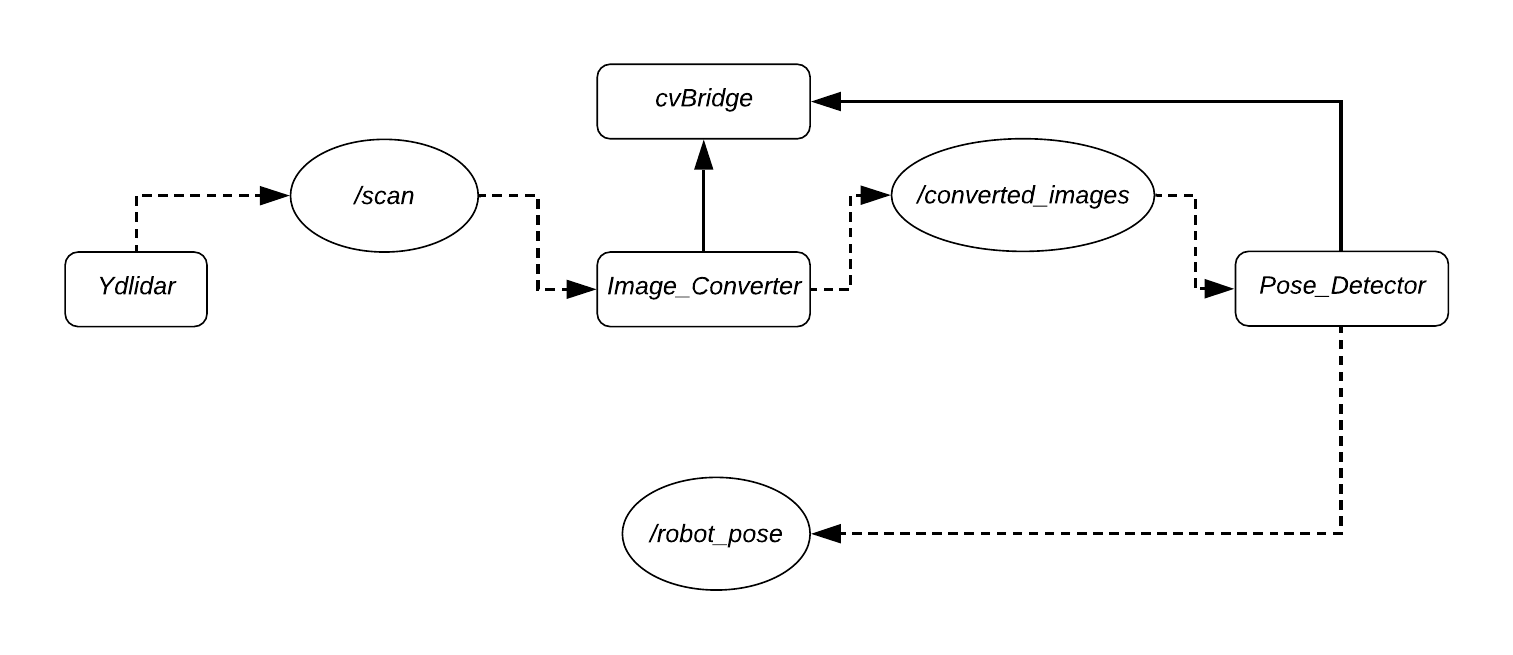
\includegraphics[width = 1\textwidth, frame]{./Bilder/compgraph2.png}
	\caption{Computational graph of OpenCV method}
	\label{fig10}
\end{figure}

The laser scanner generates a 2D point cloud, which is the content of the LaserScann Message. In this message, a measured distance is assigned for each scan angle. The ImageConverter node converts this point cloud into a 2x2 matrix, which is a binary image matrix. The pixels of the image matrix with the value "True" correspond to the XY-coordinates of the points in the point cloud.\\
To simplify the implementation of the ImageConverter node, the following activity diagram shown in figure \ref{fig11} was designed.
\begin{figure}[ht]
	\centering
	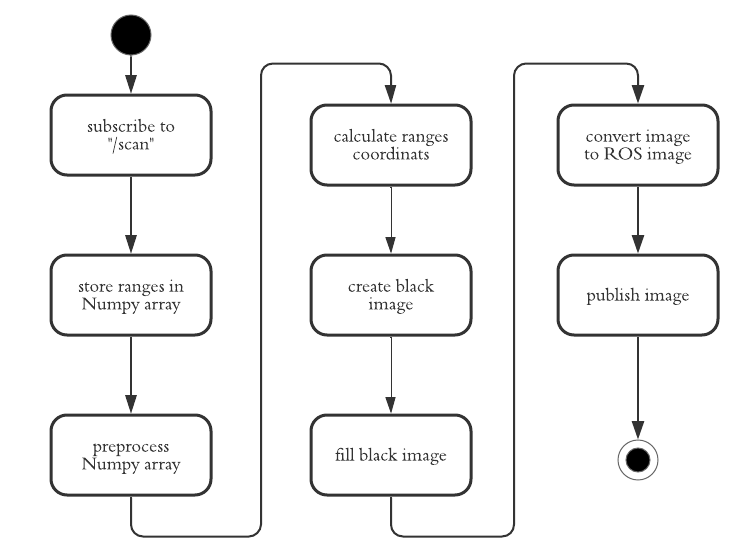
\includegraphics[width = 0.7\textwidth, frame]{./Bilder/activity.png}
	\caption{Activity diagram of the ImageConverter node}
	\label{fig11}
\end{figure}
This step is essential to understand the flow control of the node. First, it subscribes to the "scan" topic to get the ranges of the LaserScan message. Then, the ranges are stored in a numpy array. Since some ranges may have invalid values, the ranges array must be preprocessed to delete these values. The next step is to calculate the exact position of each range in the XY plane. This can be done as follows:\\
Since the angle increment $i$ of the laser scanner is known, then the position of each range can be represented as a point in polar coordinates as $(r_n,\theta_n)$, where $n \subset [0, \frac{360�}{i}]$. This point can be represented in Cartesian coordinates as $(x_n,y_n)$ where:
\begin{equation}\label{eq11}
x_n = r_n \cdot cos(\theta_n), \hspace{3mm} y_n = r_n \cdot sin(\theta_n)
\end{equation}
By vectorizing the previous formula, the coordinates of each range point in XY plane can be represented as follows:

\begin{equation}\label{eq12}
 \begin{pmatrix}
    x_0\\
    \cdots\\
    x_n
 \end{pmatrix} =
\begin{pmatrix}
    r_0 cos(\theta_0)\\
    \vdots\\
    r_n cos(\theta_n)
\end{pmatrix}, \hspace{3mm}
  \begin{pmatrix}
    y_0\\
    \cdots\\
    y_n
 \end{pmatrix} =
\begin{pmatrix}
    r_0 sin(\theta_0)\\
    \vdots\\
    r_n sin(\theta_n)
\end{pmatrix}
\end{equation}

The next step is to create a blank black image using OpenCV. After that being done, the color of corresponding pixels in this image to the positions from equation \ref{eq12} must be changed. As Pixels are integer values, the positions calculated in \ref{eq12} must be changed to integer values. This process has intelligibly a huge impact on the resolution of the localization process. To explain this impact, the following example is considered. Assuming the points $P_1$ and $P_2$, which are detected from the cylinder are next to each other, where $a$ is the distance between those points. According to \ref{eq10}, $a = 0.018$ m, when the cylinder is detected by 10 points. Thus, it follows that the resolution of the image must be at least $1 \frac{pixel}{mm}$. Since the room width and length are 1.5 \si{\meter}, then The size of the image can be calculated as follows:
\begin{equation*}\label{eq13}
\text{image size} = Resolution� \cdot width \cdot length   = 2250 \cdot 10� \text{ pixels}
\end{equation*}

The next step in the activity diagram in figure \ref{fig11} is to convert the openCV image into ROS image. The last step is then to publish the ROS image at a proper rate. Since, the Ydlidar laser scanner publishes LaserScan messages at rate of 20 \si{\hertz}, the rate of this node must be greater than 20 \si{\hertz}. This means each image must be processed withn 50 ms. This is a very short time to process the images and localize the robot. Thus, this approach is not used for localizing the robot. However, using image processing approach could be useful, if a camera is used instead of the laser scanner. By using a camera, objects would be easier to detect directly. 
 


\subsection{Laser Scan Matcher} %4 pages
%1)introduction and explain how the algorithm work
%2)how to implement the laser scan matcher. which data are used as inputs and %what is the output of the algorithm (Computational graph)
%3) Difficulties, and why didn't I continue working on this approach


Another approach to localize the pose of the robot is using the Canonical Scan Matcher (CSM) implementation. The CSM is a library in C that is used for scan matching problems, i.e., in mobile robot applications, and was developed by Andrea Censi \cite{censi_csm_nodate}. As described in \cite{censi_accurate_2007}, CSM introduces a new method to compute the covariance of the ICP (Iterative Closes/Corresponding Point) algorithms, which are used for comparing different scans to each other and match these scans so that the difference between them is minimized. Fortunately, the CSM library is implemented into ROS as a package called laser scan matcher. This is the core algorithm of the well-known SLAM localization. To understand how the laser scan matcher package works, the following example is considered. Assuming a mobile robot is moving in a room, and a laser scanner is standing on the top of the robot. While the robot moves, the laser scanner scans the surrounding area and publishes scan frames. These scan frames are used as an input to the laser scan matcher node. The laser scan matcher node tries then to compare these scan frames to each other.  By comparing the scan frames repetitively, the laser scan matcher node can estimate the difference between the scan frames and determine the pose of the robot.  In this section, the implementation of the laser scan matcher package, as well as its disadvantages, are explained.

The following example is to be considered in order to understand the implementation of the laser scan matcher package. This example demonstrates the implementation of a robot, where a laser scanner is set on top of this robot and moving with it.  This is different from the approach used in this thesis, where the laser scanner and the robot are not moving together. However, it would help to understand the concept of this approach. 

According to figure \ref{fig12}, the laser scan matcher node publishes the pose of the robot to both topics tf and pose2D. For estimating the pose of the robot, the laser scan matcher node subscribes to several topics, as explained in \cite{noauthor_laser_nodate-1}.

\begin{figure}[ht]
	\centering
	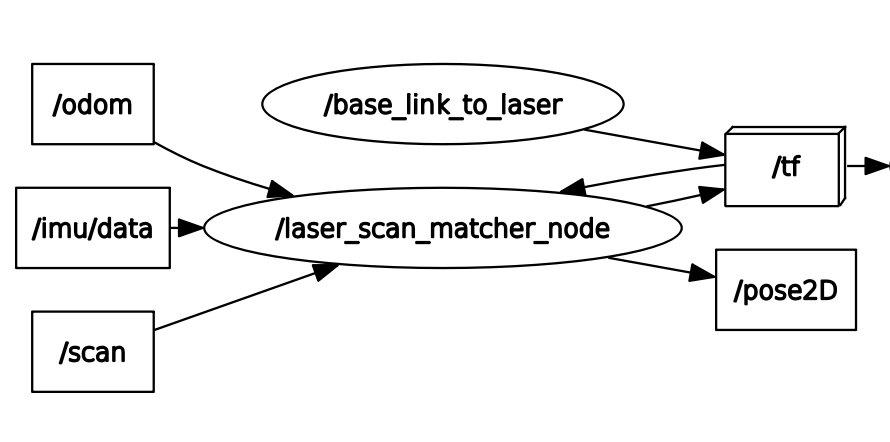
\includegraphics[width = 0.8\textwidth, frame]{./Bilder/lsmgraph.png}
	\caption{Computational graph of laser scan matcher}
	\label{fig12}
\end{figure}

The first topic is "/scan", which contains the LaserScan messages. The second topic needed for the pose calculation is  "tf". The "tf" topic contains the transformation messages between the laser scanner frame and the robot's base frame as well as the transformation messages between the robot's base frame and the world frame. The pose of the robot is computed relative to the world frame, which is a fixed frame in the map. These two topics are essential for pose calculation. However, other topics can be used to improve the accuracy of the laser scan matcher, such as 'IMU/data,' which contains data of an IMU sensor. Another topic that is used to improve the accuracy of the process is 'Odom'. This topic has the wheel odometry data, which is calculated using wheel encoders. Additionally, the  IMU sensor could be used for a more accurate calculation of the pose. However, these supplementary topics are not used in the implementation of the robot, since Legoboost robot does not have such sensors. 

The challenge momentarily is to adjust this example to fit with the aim of this thesis, where the laser scanner is not integrated into the robot.

In order for this to be done, two things must be modified. First, the fixed frame must be changed to be the laser scanner frame. Now, the pose of the robot is calculated relative to the laser scanner. The second thing is the scan messages. The laser scan matcher compares laser frames iteratively, and by matching these frames, the pose is calculated. This means that in order to calculate the pose of the robot, the scan plane must not be constant and must change.  Since the laser scanner scans both the room and the robot, and the room's scan points are constant because the laser scanner is not moving, the whole scan frame is almost constant because the scan points of the room are way more the scan points of the robot. Thus, the scan points of the room must be excluded from the scan message using scan filters, as explained in section \ref{subsec:computationGraph}. However, excluding the room points would lead to another problem, namely the very few amount of the scan points, which cannot provide the laser scan matcher with enough data to calculate the pose of the robot. Thus, this approach is not used to localize the pose of the robot.


\section{Motion Control and System Integration}

The last component in the project is the motion control algorithm. As previously mentioned, the aim of the project at the end is to build a system where the robot follows a predefined path. This path can be interpreted as a straight line, a trajectory, or even only a pose in the room.  For each kind of path, there is a specific control algorithm. The control algorithm implemented in this project is the "following a line" algorithm. However, in the future, other control algorithms can be implemented in separate nodes. This is the advantage of ROS, where all components are loosely coupled and can be implemented and activated separately. In this section, the implementation of the "following a line" algorithm is explained as described in \cite{corke_robotics_2017}. After the implementation of the motion control, the integration of the ROS system including all nodes will be discussed.\\

\subsection{Motion Control}
Since two separate motors control the robot's movement, the kinematics of a differential drive robot must be considered. As explained previously, the speeds of the individual wheels determine both the angular velocity and the linear velocity of the robot.\\
The line that the robot has to follow can be described with the following equation:


\begin{equation} \label{eq14}
ax+by+c = 0
\end{equation}

As mentioned in \cite{corke_robotics_2017}, in order to follow this line, two controllers must be considered. The first controller controls the robot's distance to the line, while the second controller controls the steering angle. The two controllers are then added together to determine the robot's overall motion, namely the speeds of the individual wheels.\\

The distance controller can be described as follows:

\begin{equation} \label{eq15}
d = \frac{(a,b,c)}{\sqrt{a�+b�}}
\end{equation}
where $d$ is the distance to the line.\\

The steering angle controller can be described as follows:
\begin{equation} \label{eq16}
\theta^* = tan^{-1}(\frac{a}{b})
\end{equation}


By adding both controllers in \ref{eq15} and \ref{eq16}, the controller can be described as follows:

\begin{equation} \label{eq17}
\alpha = -K_d +K_h \cdot (\theta^*-\theta)
\end{equation}
where \hspace{15mm} $K_d$ is the distance parameter\\ 
	  \hspace*{26mm} $K_h$ is the heading parameter

The controller in \ref{eq17} takes the position and orientation of the robot as input. The output of the controller is the angular velocity.
Using the equations \ref{eq2_2} and \ref{eq2_5}, the velocities of the right and left wheels can be calculated as follows:

\begin{equation} \label{eq18}
V_L = \frac{1-W \cdot \alpha}{R}
\end{equation}
\begin{equation} \label{eq19}
V_R = \frac{1+W \cdot \alpha}{R}
\end{equation}

The controller node is implemented in Python. It subscribes to the pose of the robot and does not publish any data. By implementing the node in Python, Python's powerful MatplotLib library can be used to plot the results.
In order to adjust the controllers' parameters, a simulation in Simulink has been developed as displayed in figure \ref{fig13}. The simulation also helps to verify the solution and is used generally for debugging purposes.\\

\begin{figure}[ht]
	\centering
	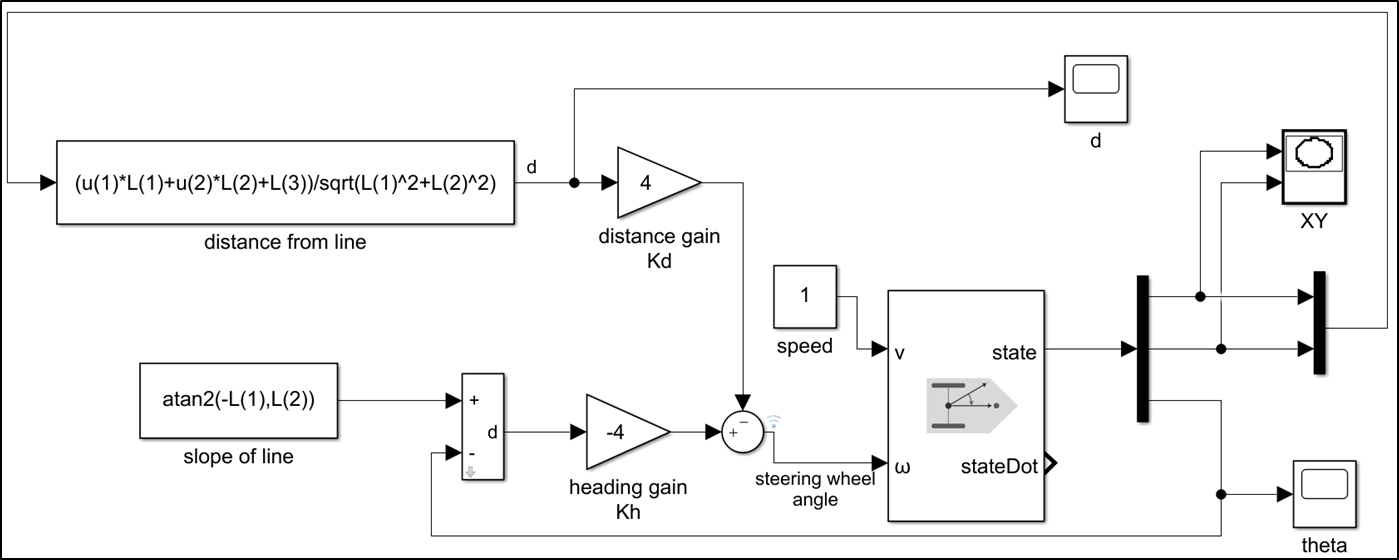
\includegraphics[width = 1\textwidth, frame]{./Bilder/Simulink.png}
	\caption{Simulation of following a line algorithm in Simulink}
	\label{fig13}
\end{figure}



\subsection{System Integration}
After implementing the controller, the final step is to integrate the system components into one system. Instead of launching each node separately in the terminal, ROS provides the possibility of launching several nodes using ROS launch files. In the ROS launch file, all nodes needed for the project will be included. This is the mastery of ROS as the user can then adjust or even extend the software. The configuration of the launch file is demonstrated in figure \ref{fig14}. Launch files are basically XML configuration files.

\begin{figure}[ht]
	\centering
	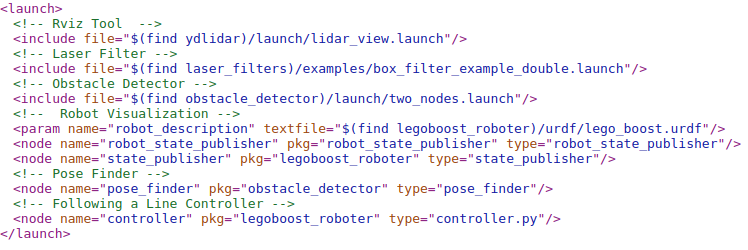
\includegraphics[width = 1\textwidth, frame]{./Bilder/XMLROS.png}
	\caption{Launch file of the system}
	\label{fig14}
\end{figure}














